\documentclass[12pt]{mitthesis} 

\usepackage{lgrind, braket, amsmath,
  amssymb, bbm, booktabs, subfig, color} 

\usepackage[pdftex]{graphicx}
\usepackage[version=3]{mhchem}

\newcommand{\TODO} [1]{\textcolor{magenta}{\textbf{TODO:} #1}}
\newcommand{\NOTE} [1]{\textcolor{magenta}{[\emph{#1}]}}
\newcommand{\POINT}[1]{\textcolor{magenta}{\textbf{POINT:} #1}}

\newcommand{\rcm}{cm$^{-1}$}
\newcommand{\bigspace}{$
  \;
  $}

\newcommand{\astate}{$
  \tilde{A} \: ^1\!A_u
  $}
\newcommand{\AtoX}{$
  \tilde{A} \: ^1\!A_u 
  \leftarrow 
  \tilde{X} \: ^1\Sigma_g^+
  $}
\newcommand{\StoS}{$
  S_1 \leftarrow S_0
  $}
\newcommand{\microsec}{$\mu$s}

% scientific notation
\newcommand{\e}[1]{\ensuremath{\times 10^{#1}}}

% temperatures
\newcommand{\degrees}{\ensuremath{^\circ}}

% hyphenation
\hyphenation{acetylene}
\hyphenation{Hamiltonian}

\begin{document}

\listoffigures
\clearpage

\listoftables
\clearpage
\subsubsection*{NOTES}
I have collected all of the data figures from chapter 4 of my thesis.
Please help me check the language, grammar, and accuracy of the
captions!  I would also appreciate suggestions on how to make the
figures communicate the main points more clearly.

Some lingering issues:

Do people prefer the $\nu'_2+2\nu'_3$ notation or the $2^13^2$
notation?  I think the former is easier to understand for
non-spectroscopists, but it is definitely the uglier of the two.

Can I get rid of some of the repeated phrases in the captions, without
changing the order of the figures?

Do I need to include legends in the figures of c.o.g. vs. time?  The
upper state quantum number is labeled to the right, but the legend may
help readers follow the lines as they cross in the plot.

Thank you, early readers!
\clearpage

\setcounter{chapter}{3}
\chapter{SEELEM/LIF spectroscopy of acetylene: Spectral signatures of
  energetically distant doorway levels}

\begin{table}
  \caption{Term values of the acetylene \astate\ vibrational levels considered in
    this study.  The energies of all four levels are in the critical
    region above the $S_1 \sim T_3$ electronic seam of intersection
    ($\simeq 45300$ \rcm) but below the first dissociation barrier
    ($\simeq 46300$ \rcm).}
  \label{table:termvals}
  \centering
  \begin{tabular}{llr}
    Level & & Term value (\rcm ) \\
    \midrule
    $2\nu_2' +  \nu_3'$ & $K_a$=1 & 46010 \\
    $2\nu_3' + 2\nu_4'$ & $K_a$=1 & 45812 \\
    $ \nu_2' + 2\nu_3'$ & $K_a$=1 & 45677 \\
    $3\nu_3'          $ & $K_a$=2 & 45352 \\
  \end{tabular}
\end{table}

\section{$\nu'_2+2\nu'_3$}

\begin{figure}
  \caption{Simultaneously recorded SEELEM (upper trace) and LIF (lower
    trace) spectra of the $\nu_2'+2\nu_3'$ $K_a$=1 sublevel of the
    $\tilde{A}^1A_u \leftarrow \tilde{X} ^1\Sigma_g^+$ electronic
    transition.  The LIF spectrum is integrated in two time regions:
    an early time window ($0.5\tau_s-2\tau_s$, solid trace) and a
    delayed time window ($10\tau_s-18\tau_s$, dashed trace).  The
    Q(1) and Q(2) transitions are redshifted in the delayed
    fluorescence spectrum, in contrast to the Q(3,4,5) transitions.
    The P(2) transition, having the same $J'$ but opposite parity from
    Q(1), shows a similar redshift in the delayed fluorescence
    spectrum.}
  \label{fig:spectrum-2132}
  \centering
  \vspace{1cm}
  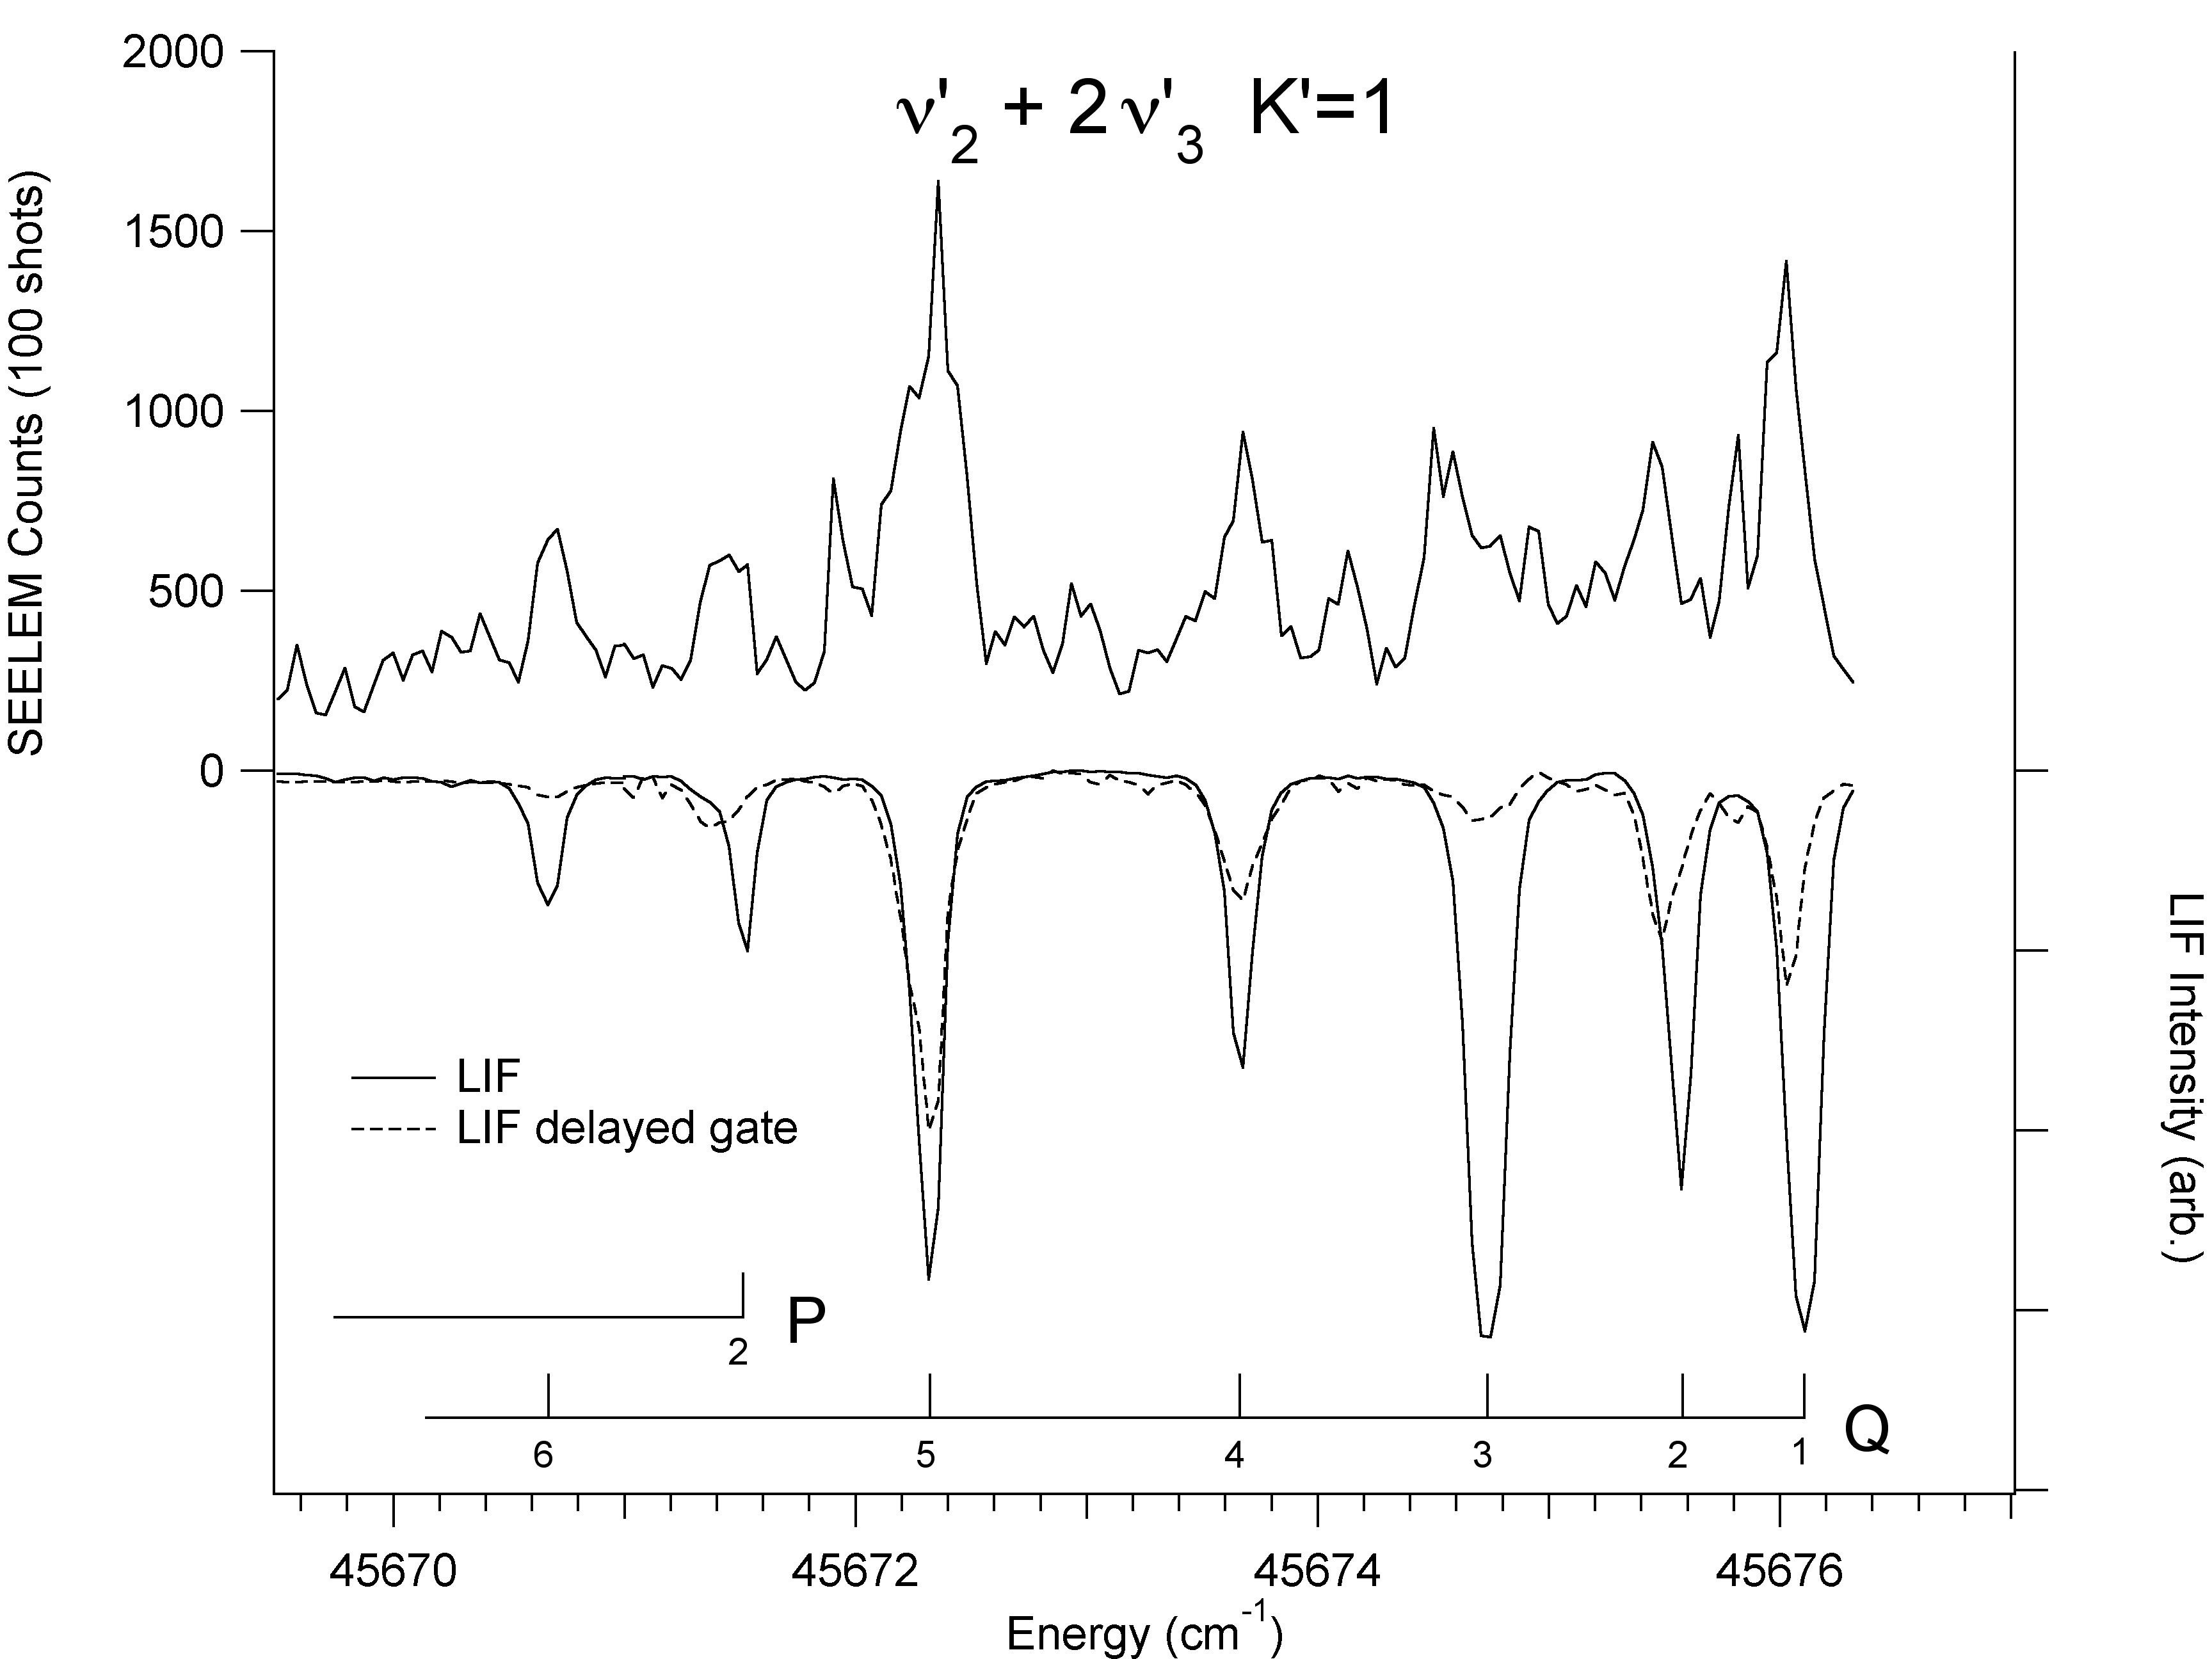
\includegraphics[width=7in,angle=90]{acetylene-2132-q6q1.png}
\end{figure}

\begin{figure}
  \caption{Dependence of the intensity-weighted center of gravity on
    delay for a series of individually resolved transitions, Q(1$-$5),
    in the LIF spectrum of the $\nu_2'+2\nu_3'$ $K_a$=1 sublevel.  The
    Q(1) and Q(2) transitions arrive at peak positions identical to
    the those in the SEELEM spectrum by a delay of $15\tau_s$.}
  \label{fig:2132-q123456-cog-delay}
  \centering
  \vspace{1cm}
  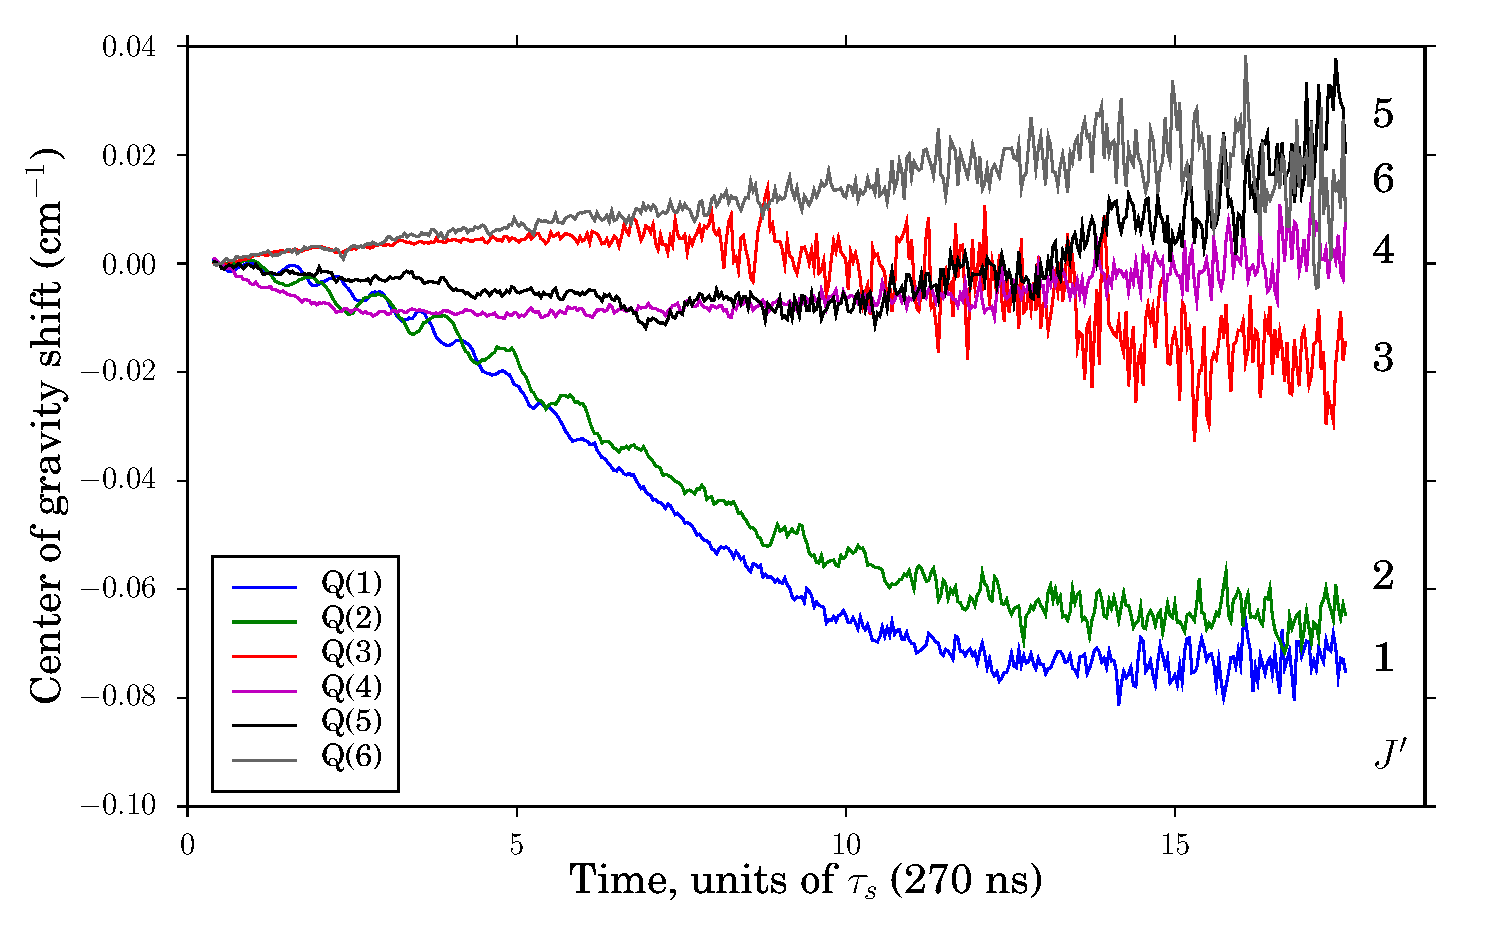
\includegraphics[width=6in]{2132-q123456-cog-delay.pdf}
\end{figure}

\section{$2\nu'_2+\nu'_3$}

\begin{figure}
  \caption{Simultaneously recorded SEELEM (upper trace) and LIF (lower
    trace) spectra of the $2\nu'_2+\nu'_3$ $K'_a\!=\!1$ sublevel of the
    $\tilde{A}^1A_u \leftarrow \tilde{X} ^1\Sigma_g^+$ electronic
    transition.  The LIF spectrum is integrated in two time regions:
    an early time window ($0.5\tau_s-2\tau_s$, solid trace) and a
    delayed time window ($8\tau_s-12\tau_s$, dashed trace).  The Q(1)
    and R(0) transitions, which have the same upper state quantum
    number $J'=1$ but different parities, are shifted to opposite
    directions in the delayed fluorescence spectrum.}
  \label{fig:spectrum-2231}
  \centering
  \vspace{1cm}
  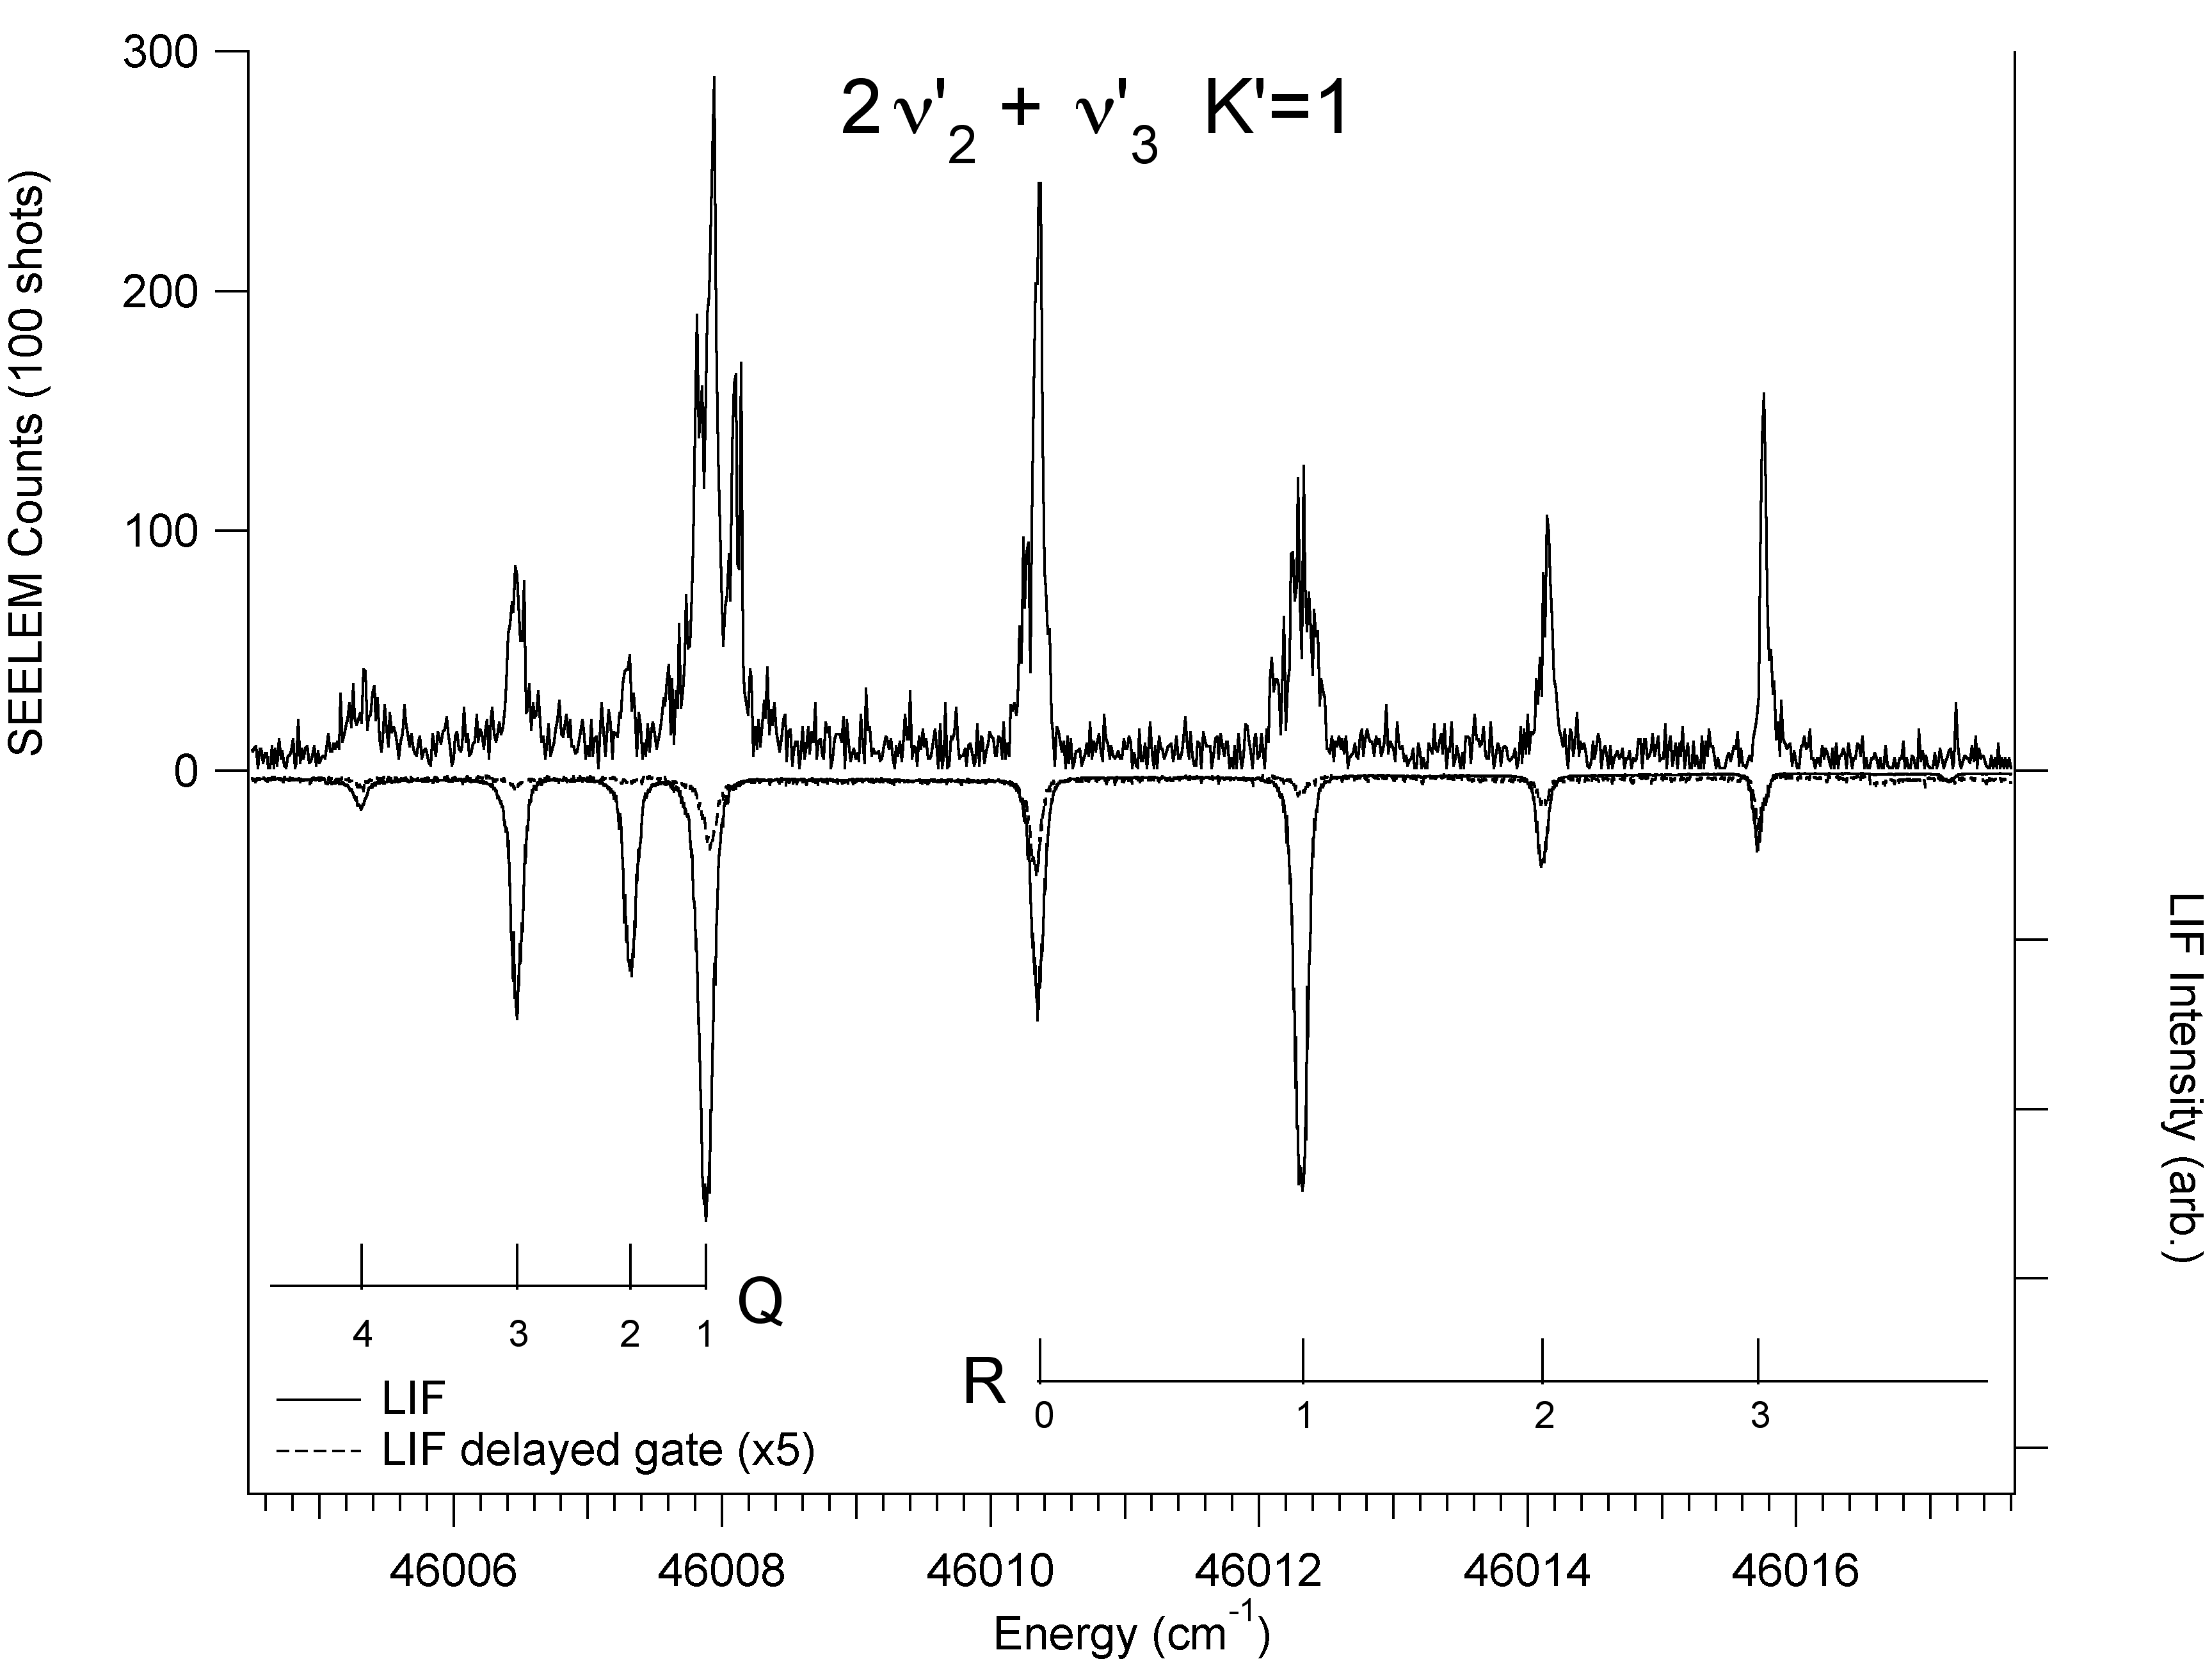
\includegraphics[width=7in,angle=90]{acetylene-2231-q4r3.png}
\end{figure}

\begin{figure}
  \caption{Dependence of the intensity-weighted center of gravity on
    delay for a series of individually resolved transitions, Q(1$-$4)
    (top), and R(0$-$3) (bottom), in the LIF spectrum of the
    $2\nu_2'+\nu_3'$ $K_a$=1 sublevel.  The center of gravity for the
    Q(1) transition rapidly increases to its final value, where it
    matches the peak of the SEELEM distribution at 46007.87$+$0.03
    \rcm.  For the R(0) transition, the center of gravity decreases at
    a nearly linear rate to 46010.35$-$0.3 \rcm.}
  \label{fig:2231-cog-delay}
  \centering
  \vspace{5mm}
  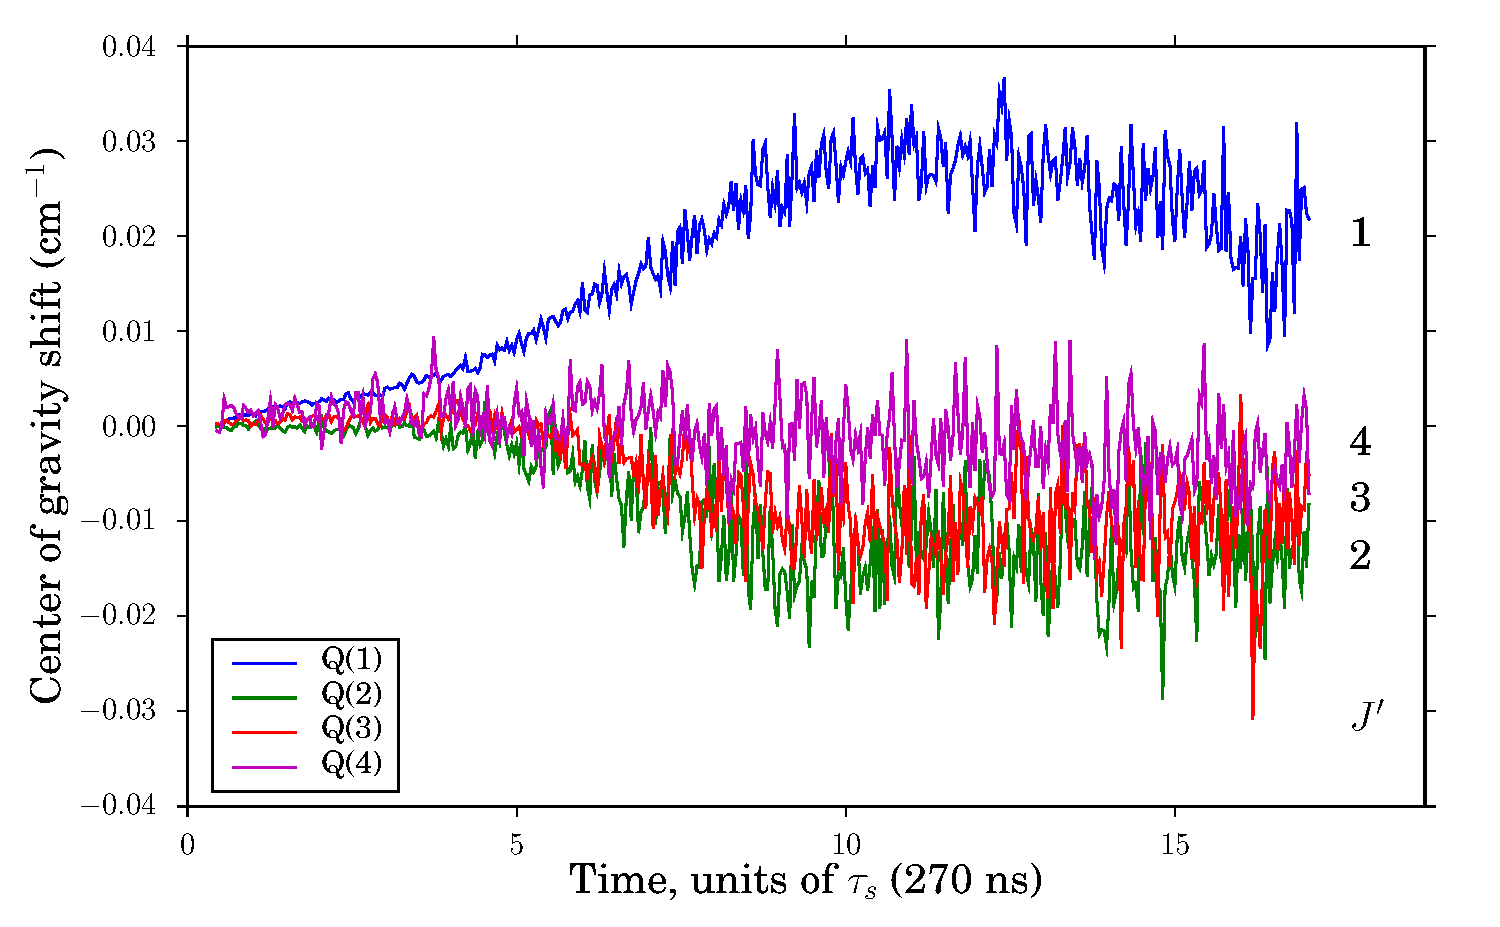
\includegraphics[width=6in]{2231-q1234-cog-delay.pdf}
  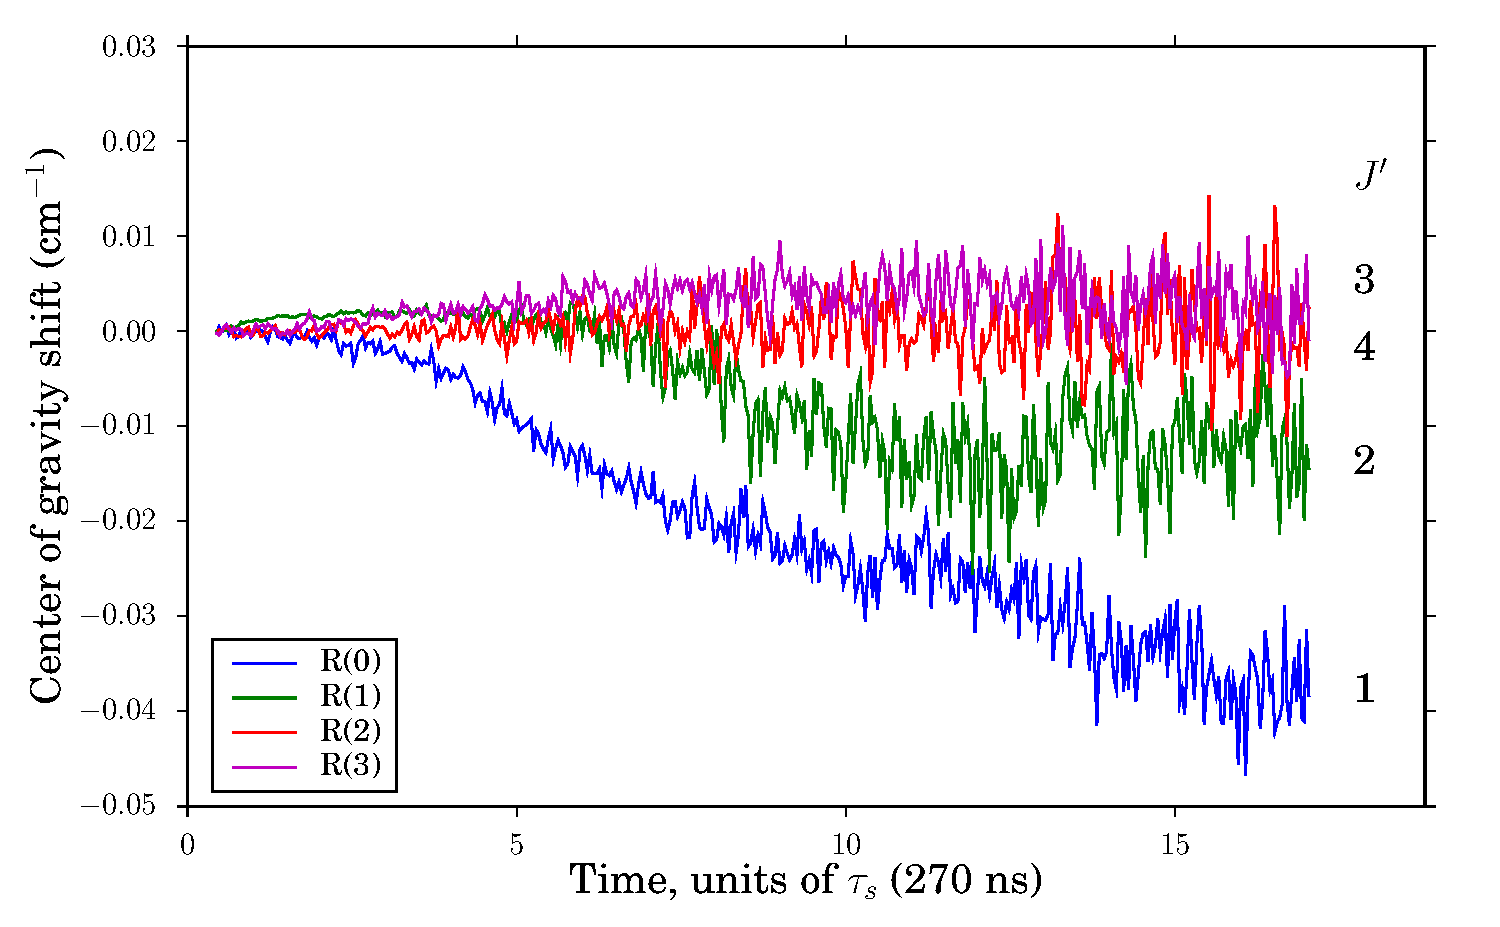
\includegraphics[width=6in]{2231-r0123-cog-delay.pdf}
\end{figure}

\begin{figure}
  \caption{[NOT TO BE INCLUDED IN FINAL CHAPTER] Simultaneously
    recorded SEELEM (upper trace) and LIF (lower trace) spectra of the
    $2\nu'_2+\nu'_3$ $K_a$=1 sublevel of the $\tilde{A}^1A_u
    \leftarrow \tilde{X} ^1\Sigma_g^+$ electronic transition, recorded
    at approximately 4$\times$ smaller energy intervals.  The LIF
    spectrum is integrated in two time regions: an early time window
    (UNSPECIFIED, solid trace) and a delayed time window (UNSPECIFIED,
    dashed trace).  The peak of the Q(1) transition is blueshifted in
    the delayed fluorescence spectrum, in contrast to the Q(2) and
    Q(3) transitions, which show essentially no shift.}
  \label{fig:spectrum-2231-q123}
  \centering
  \vspace{1cm}
  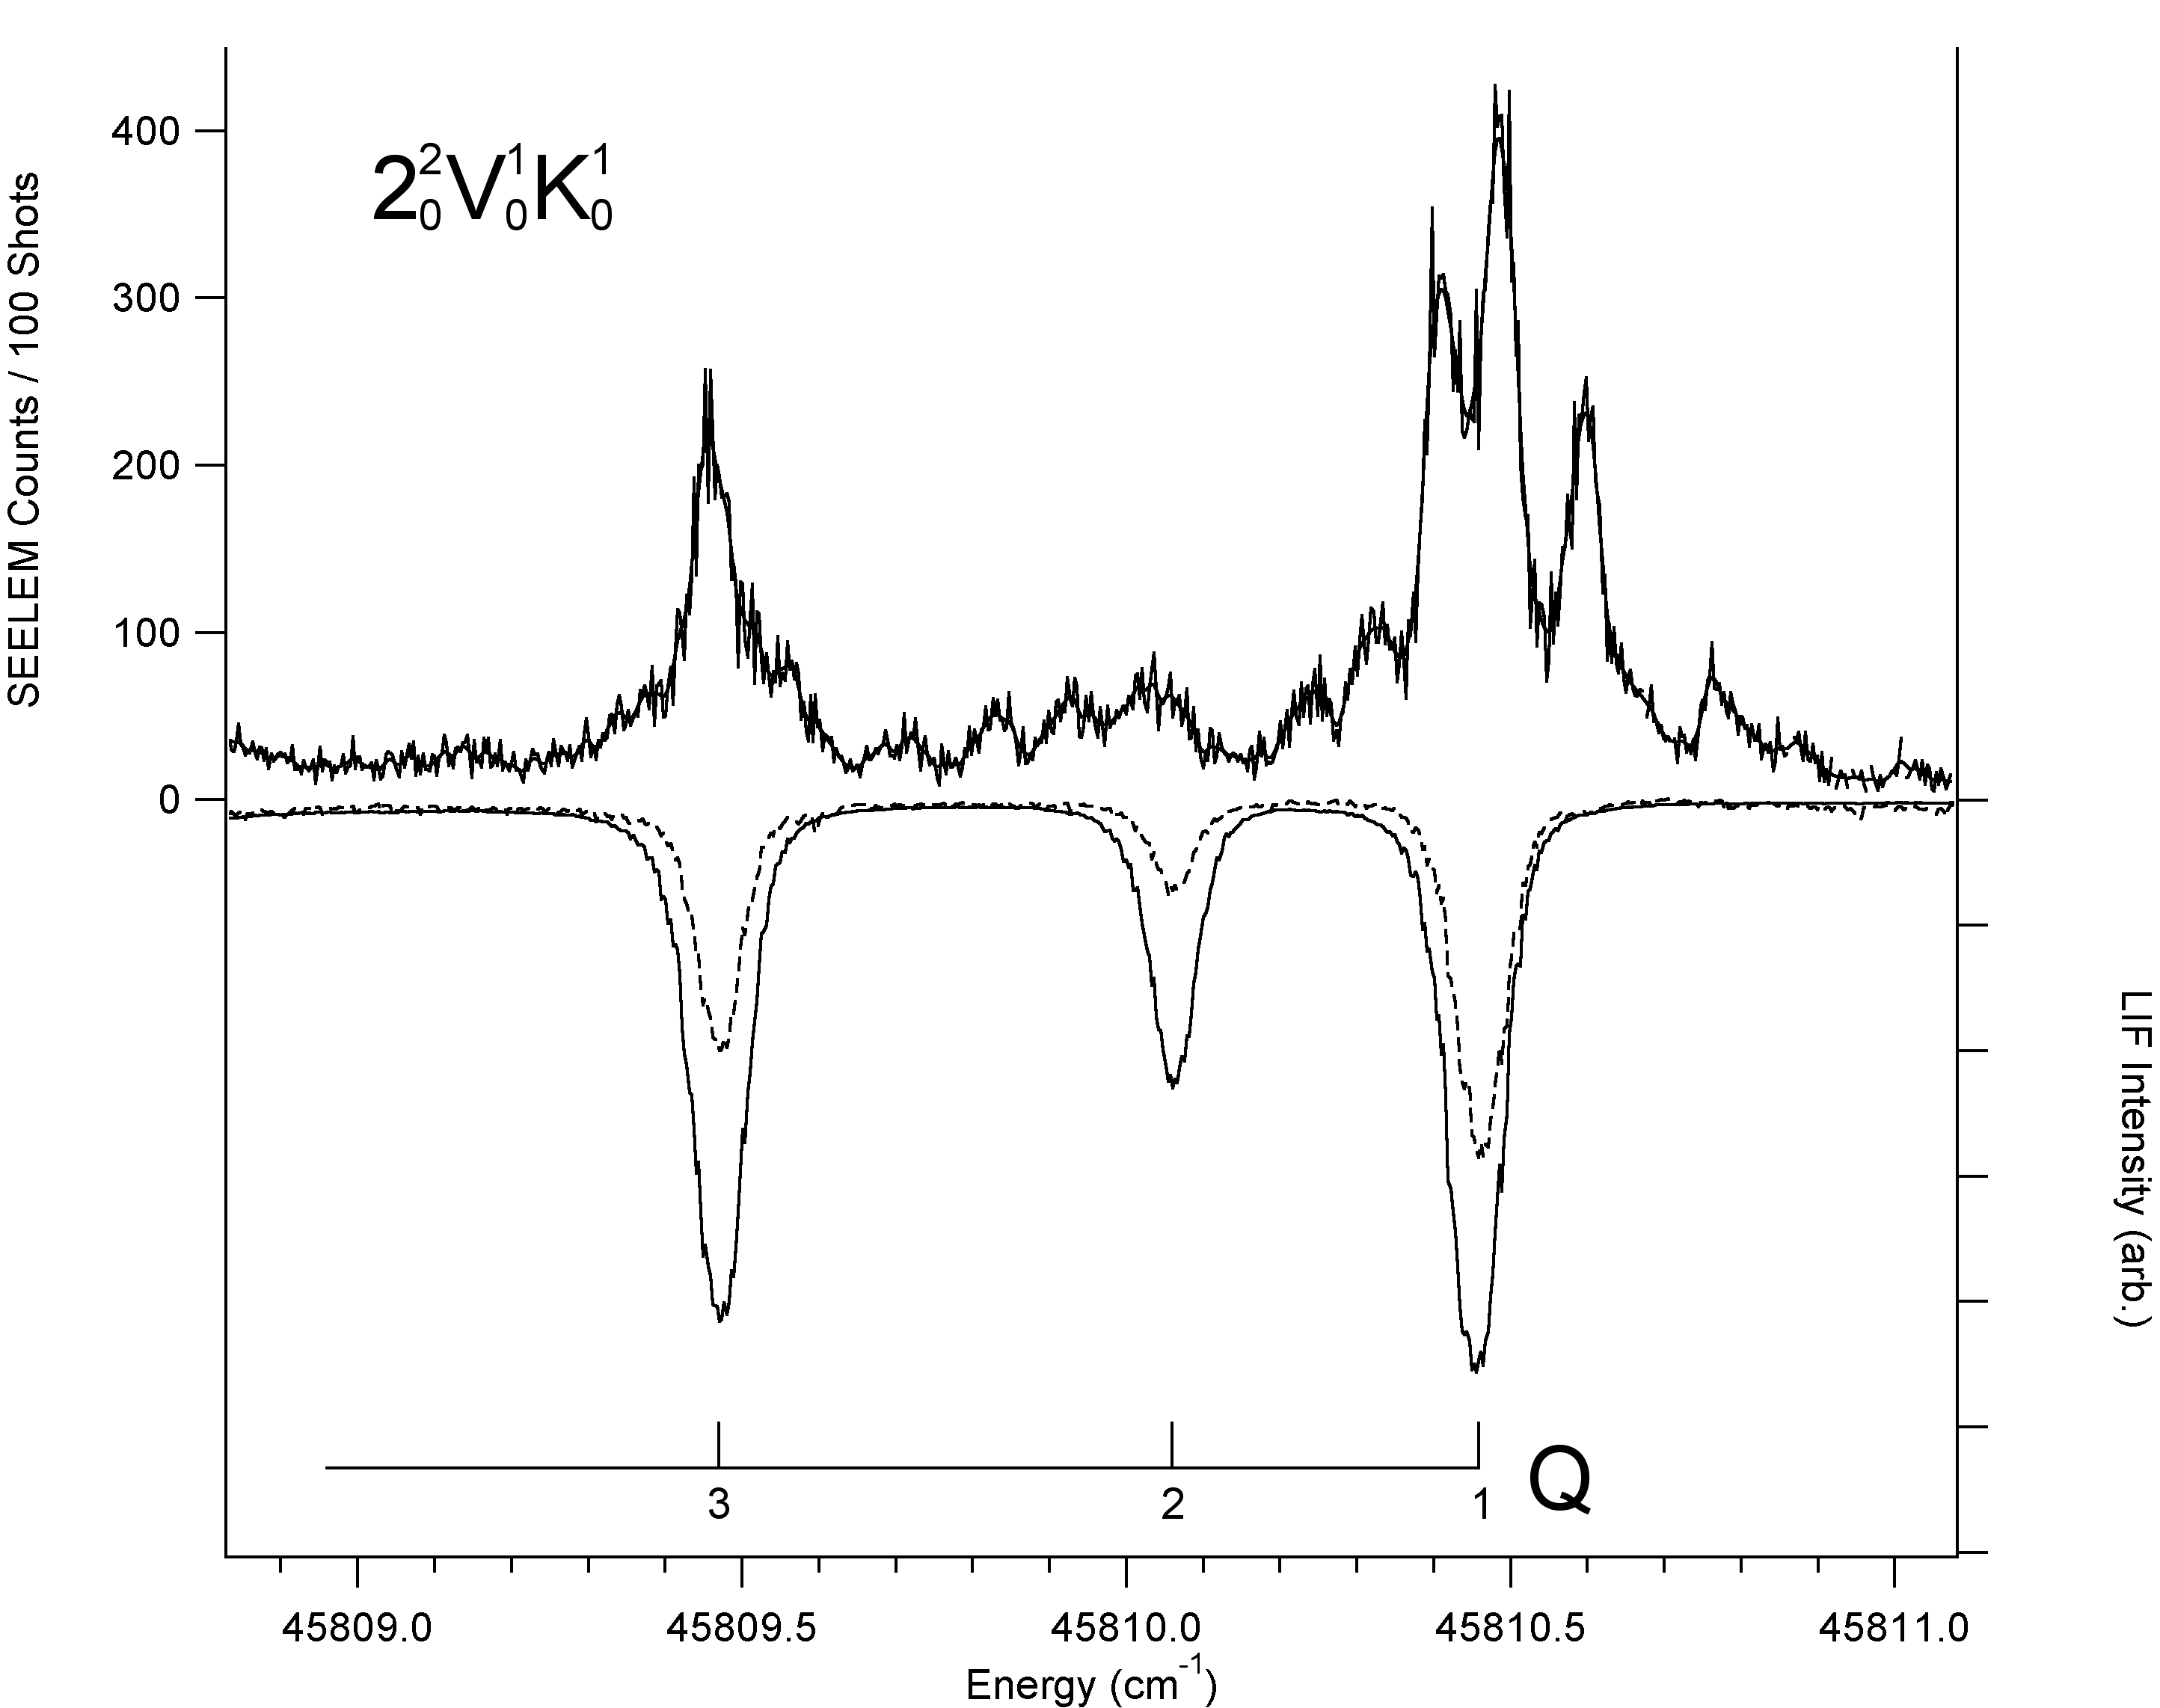
\includegraphics[width=6in]{spectrum-2231-Q123.png}
\end{figure}

\begin{figure}
  \caption{[NOT TO BE INCLUDED IN FINAL CHAPTER] Simultaneously
    recorded SEELEM (upper trace) and LIF (lower trace) spectra of the
    $2\nu'_2+\nu'_3$ $K_a$=1 sublevel of the $\tilde{A}^1A_u \leftarrow
    \tilde{X} ^1\Sigma_g^+$ electronic transition, recorded at
    approximately 4$\times$ smaller energy intervals.  The LIF
    spectrum is integrated in two time regions: an early time window
    (UNSPECIFIED, solid trace) and a delayed time window (UNSPECIFIED,
    dashed trace).  The peak of the Q(1) transition is blueshifted in
    the delayed fluorescence spectrum, in contrast to the R(0)
    transition, which is redshifted.}
  \label{fig:spectrum-2231-q1r0}
  \centering
  \vspace{1cm}
  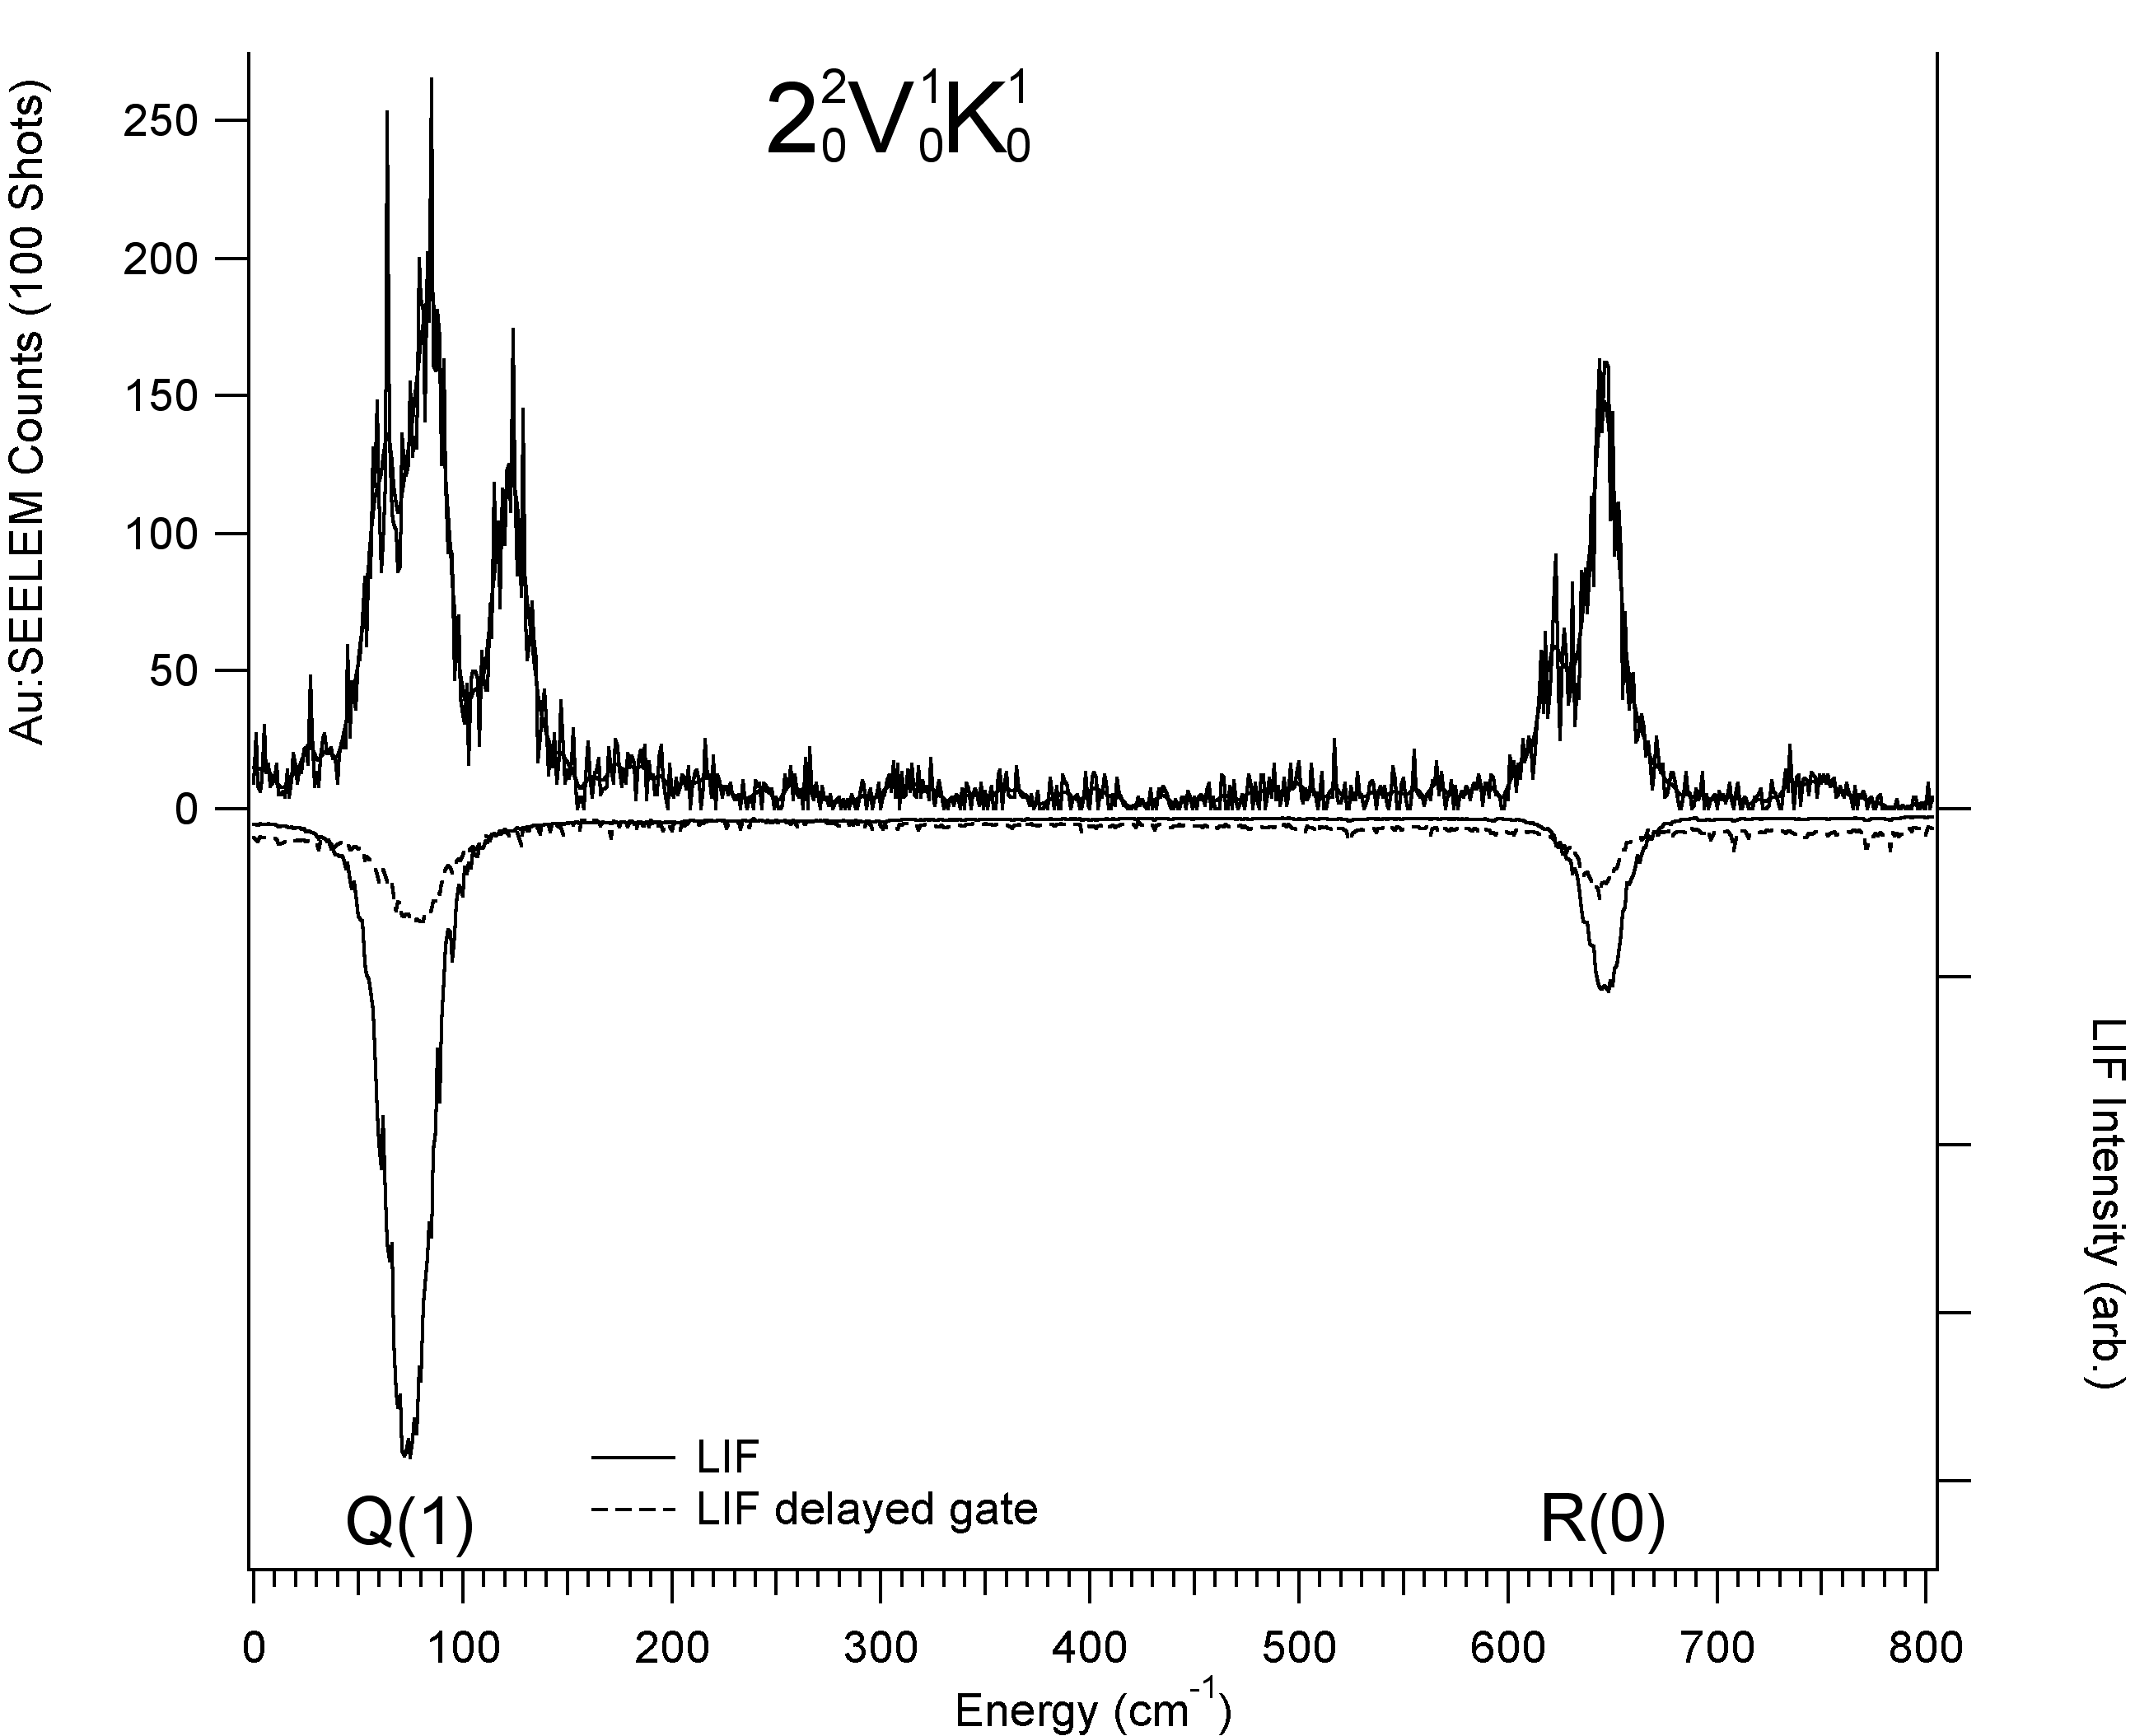
\includegraphics[width=6in]{spectrum-2231-Q1R0.png}
\end{figure}

\section{$3\nu_3'$ $K_a'\!=\!2$}

\begin{figure}
  \caption{Simultaneously recorded SEELEM (upper trace) and LIF (lower
    trace) spectra of the $3\nu_3'$ $K_a'\!=\!2$ sublevel of the
    $\tilde{A}^1A_u \leftarrow \tilde{X} ^1\Sigma_g^+$ electronic
    transition.  The LIF spectrum is integrated in two time regions:
    an early time window ($0.5\tau_s-2\tau_s$, solid trace) and a
    delayed time window ($10\tau_s-18\tau_s$, dashed trace).  The
    individual transitions are each split at least two strongly mixed
    components.  Although the energy splitting between the components
    is on the order of the experimental resolution, they are
    discernable via changes in the fluorescence lineshape resulting
    from their differing relative intenities in the early and delayed
    fluorescence spectra.  One splitting in the R(4) transition is
    just resolved in this spectrum.  \TODO{Determine the assignment for
    the set of overlapping transitions.}}
  \label{fig:spectrum-33k2}
  \centering
  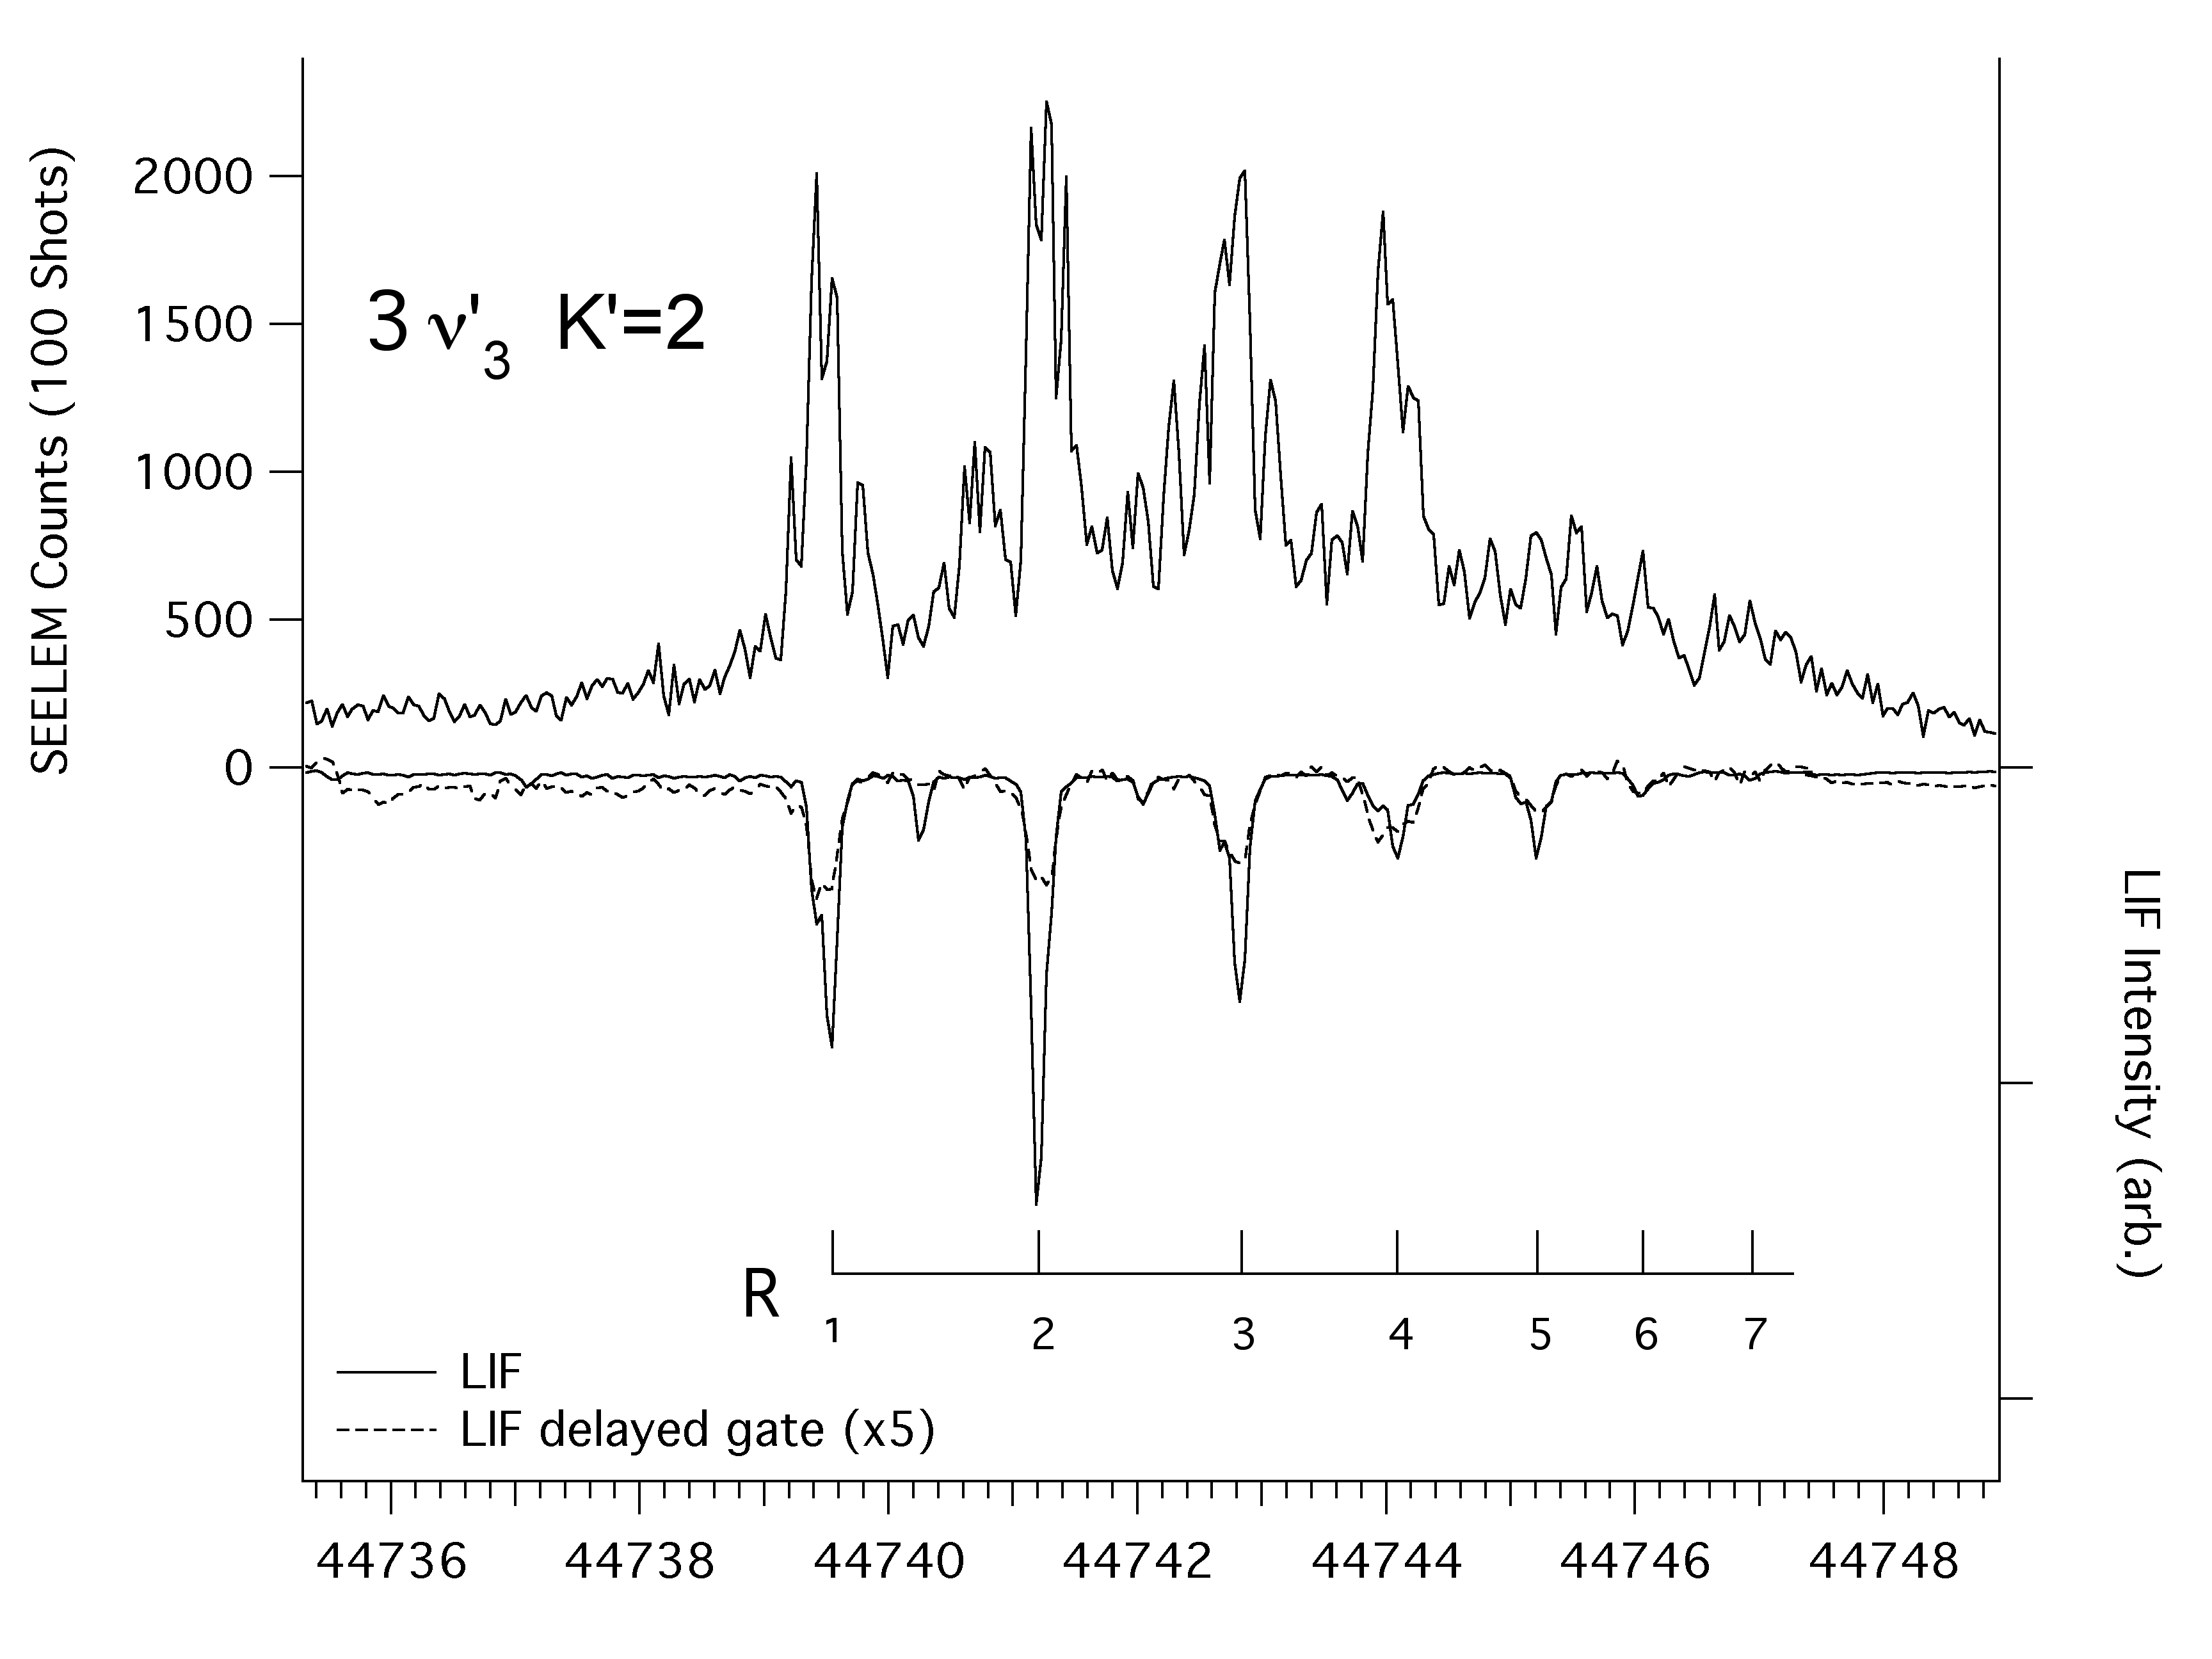
\includegraphics[width=7in,angle=90]{acetylene-33k2-r1r7.png}
\end{figure}

\begin{figure}
  \caption{Dependence of the intensity-weighted center of gravity on
    delay for a series of individually resolved transitions, R(1$-$7),
    in the LIF spectrum of the $3\nu_3'$ $K_a'\!=\!2$ sublevel.  The
    individual transitions have an overall bias to lower energies at
    long delay times, indicating an interaction with a $T_3$ doorway
    level at lower energy.}
  \label{fig:33k2-r123456-cog}
  \centering
  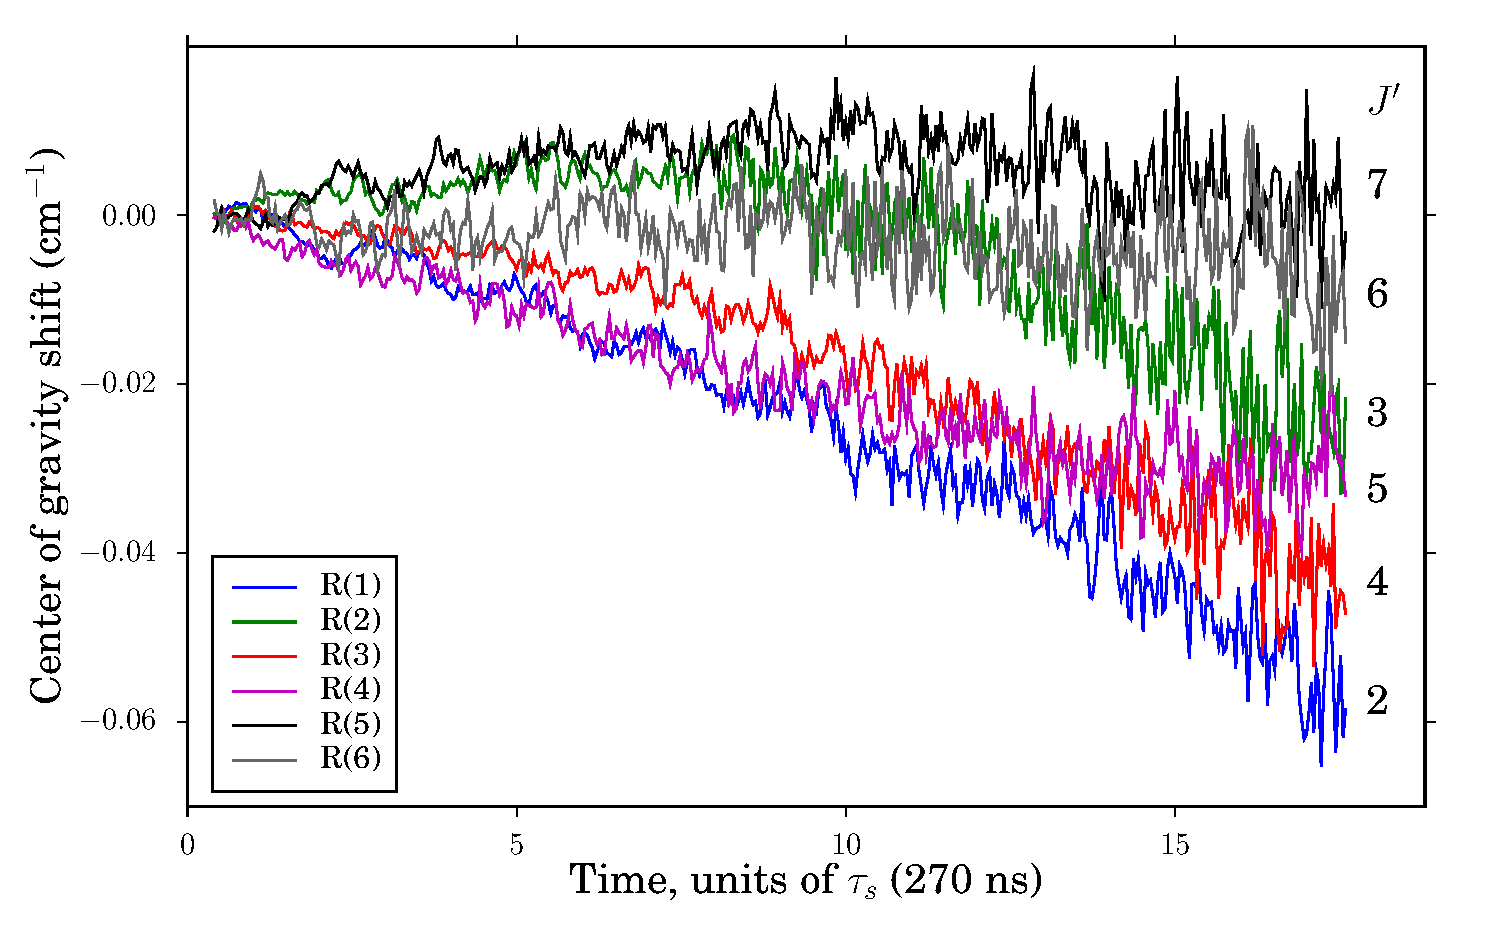
\includegraphics[width=6in]{33k2-r123456-cog-delay.pdf}
\end{figure}


\section{$2\nu'_3+2\nu'_4$}

\begin{figure}
  \caption{Simultaneously recorded SEELEM (upper trace) and LIF (lower
    trace) spectra of the $2\nu'_3+2\nu'_4$ $K'_a\!=\!1$ sublevel of
    the $\tilde{A}^1A_u \leftarrow \tilde{X} ^1\Sigma_g^+$ electronic
    transition.  The LIF spectrum is integrated in two time regions:
    an early time window ($0.5\tau_s-2\tau_s$, solid trace) and a
    delayed time window ($10\tau_s-18\tau_s$, dashed trace).  The peak
    positions are blueshifted in the delayed fluorescence spectrum for
    all transitions, with the exception of Q(2).  Perturbations from a
    level of slightly lower energy are apparent in the delayed
    fluorescence spectrum of the Q(2) and R(1) transitions.}
  \label{fig:spectrum-32b2}
  \centering
  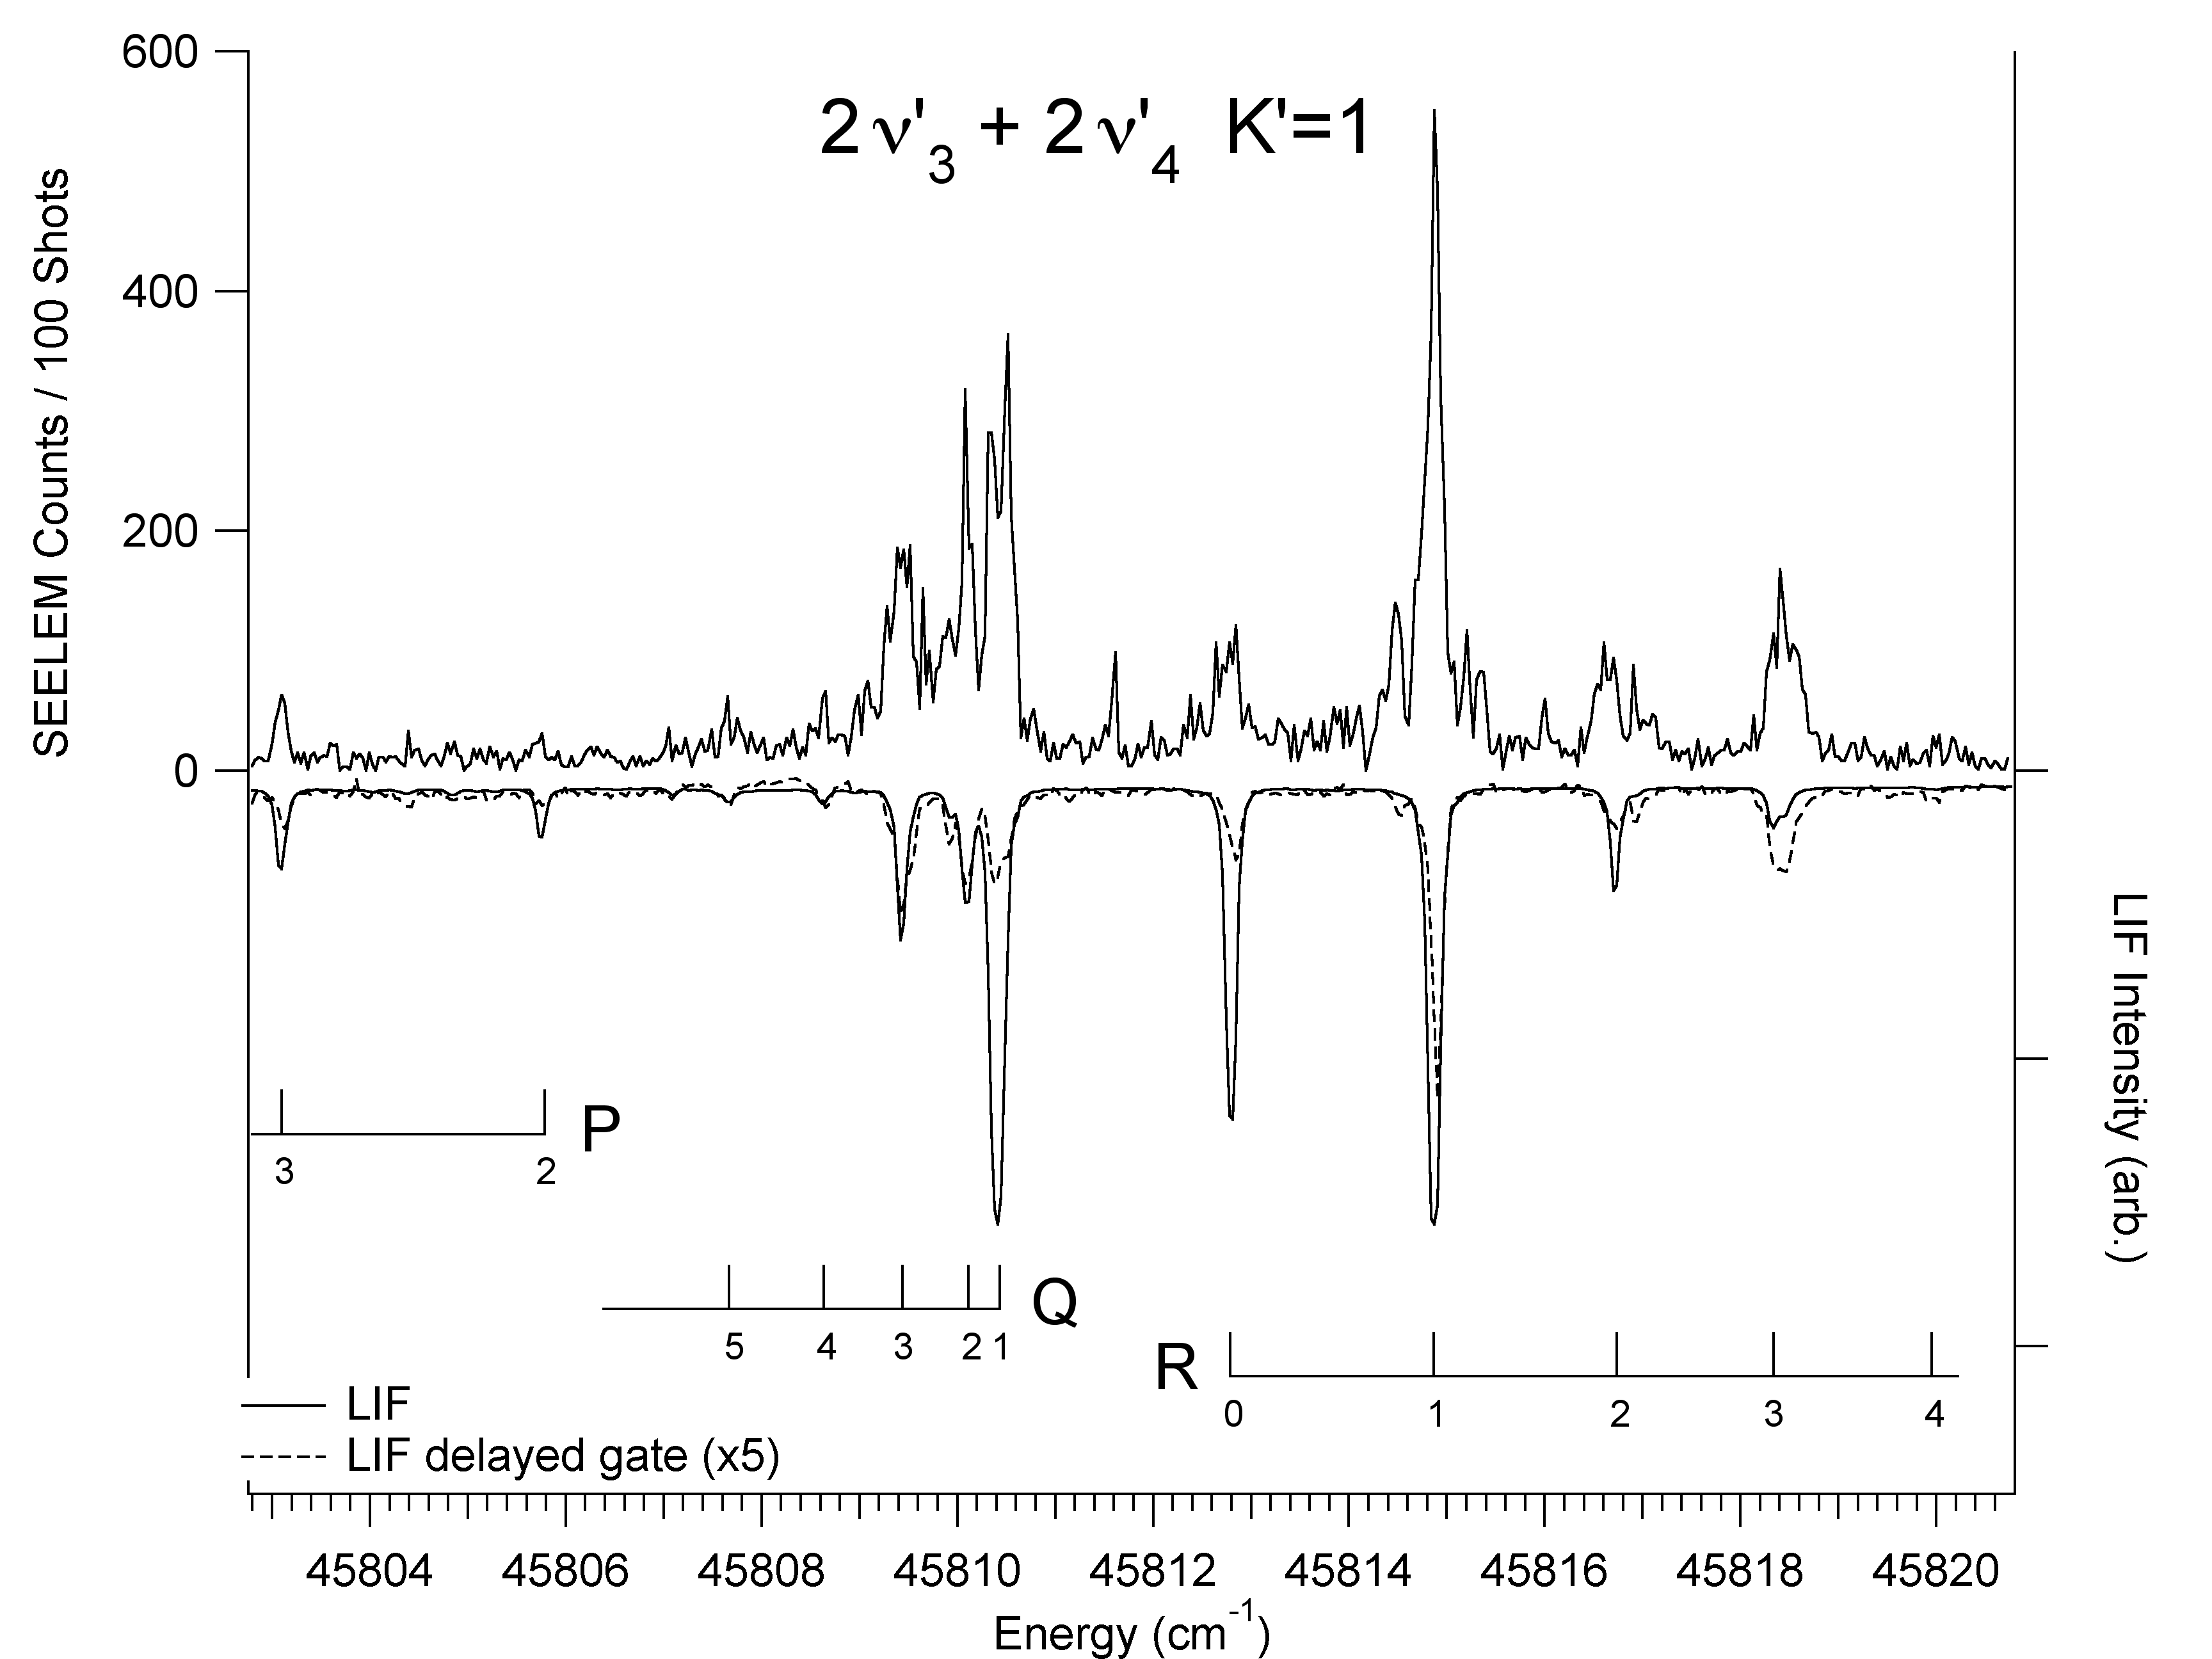
\includegraphics[width=7in,angle=90]{acetylene-32b2-p3r4.png}
\end{figure}

\begin{figure}
  \caption{Dependence of the intensity-weighted center of gravity on
    delay for a series of individually resolved transitions, Q(1$-$3)
    (top), and R(0$-$3) (bottom), in the LIF spectrum of the
    $2\nu'_3+2\nu'_4$ $K'_a\!=\!1$ sublevel.  Perturbations in the
    Q(2) and R(1) transitions cause the center of gravity to deviate
    from that of the other transitions as the delay time is increased.}
  \label{fig:32b2-cog-delay}
  \centering
  \vspace{5mm}
  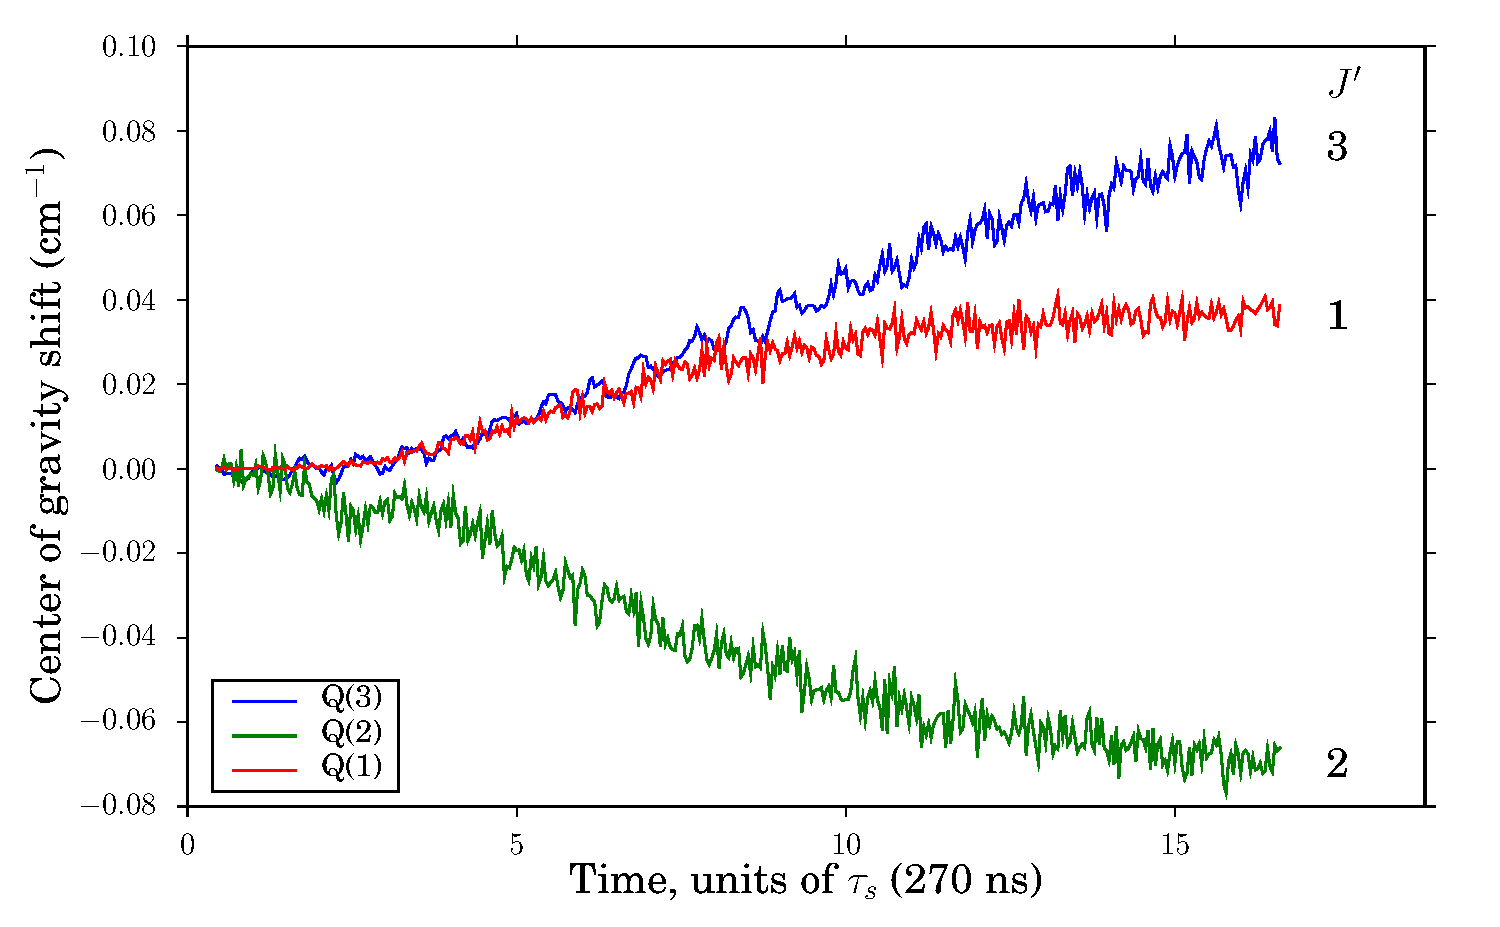
\includegraphics[width=6in]{32b2-q123-cog-delay.pdf}
  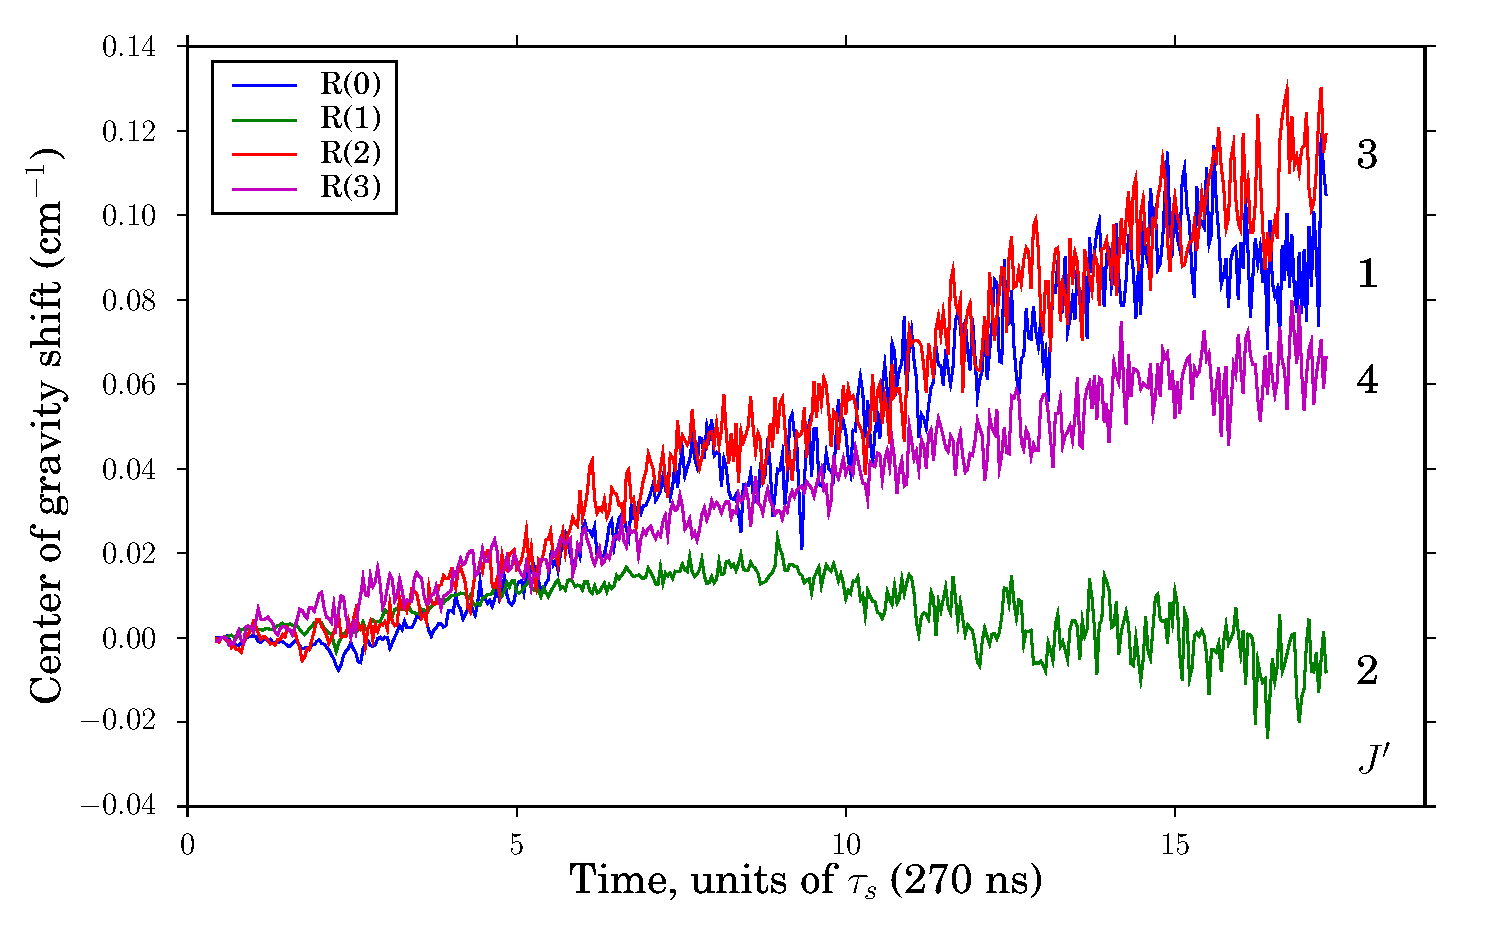
\includegraphics[width=6in]{32b2-r0123-cog-delay.pdf}
\end{figure}

\section{Band integrated center-of-gravity}

\begin{table}
  \caption{Band-integrated center of gravity measurements from
    simultaneously recorded SEELEM/LIF spectra of \astate\ acetylene.
    The SEELEM$-$LIF center of gravity is offset to lower energy for
    Q-branch measurements and offset to higher energy for R-branch measurements,
    indicating an overall increase in relative SEELEM:LIF intensity
    with $J'$.  Such $J'$-dependent behavior is predicted in the
    presence of energetically distant $T_3$ doorway levels.}
  \label{table:integrated-cog-shifts}
  \centering
        \begin{tabular}{lllll}
        \\[1cm]
        \multicolumn{3}{l}{Q-branch measurements} \\
        \toprule
        Level & Integration region & \multicolumn{2}{l}{Center of gravity} & Offset \\
        \cmidrule{3-5}
        & & LIF & SEELEM & SEELEM$-$LIF \\
        \midrule
        $\nu'_2+2\nu'_3$ & 45671.75$-$76.30 & 45674.60 & 45674.09 & $-0.51$ \\
        $2\nu'_2+\nu'_3$ & 46004.50$-$08.50 & 46007.29 & 46007.23 & $-0.06$ \\
        $2\nu'_3+2\nu'_4$ & 45807.30$-$11.00 & 45810.09 & 45809.72 & $-0.37$ \\
        \bottomrule
        \end{tabular}

        \begin{tabular}{lllll}
        \\[1cm]
        \multicolumn{3}{l}{R-branch measurements} \\
        \toprule
        Level & Integration region & \multicolumn{2}{l}{Center of gravity} & Offset \\
        \cmidrule{3-5}
        & & LIF & SEELEM & SEELEM$-$LIF \\
        \midrule
        $2\nu'_2+\nu'_3$ & 46009.50$-$16.50 & 46012.11 & 46012.49 & $+0.38$ \\
        $3\nu'_3 \:\; K'\!=\!2$ & 44738.50$-$47.50 & 44741.79 & 44742.67 & $+0.88$ \\
        $2\nu'_3+2\nu'_4$ & 45812.00$-$20.50 & 45814.67 & 45815.57 & $+0.89$ \\
        \bottomrule
        \end{tabular}
\end{table}


\end{document}
% LocalWords:  redshifted blueshifted
